\documentclass[10pt,a4paper]{article}
\usepackage[utf8]{inputenc}
\usepackage[T1]{fontenc}
\usepackage[spanish]{babel}
\usepackage{amsmath}
\usepackage{amsfonts}
\usepackage{amssymb}
\usepackage{graphicx}
\usepackage[left=1.00cm, right=1.00cm, top=2.00cm, bottom=2.00cm]{geometry}
\begin{document}
\section{Amplitud Modulada}
Es el proceso de cambiar la amplitud de una señal portadora de frecuencia relativamente alta, en proporción con el valor instantáneo de la señal modulante o moduladora. La modulación de amplitud es una forma de modulación relativamente poco costosa y de baja calidad, que se usa para emisiones comerciales de señales de audio y video.
\\
La portadora se representa con la expresión:
\begin{align}
	V_c\sin(2\pi f_c t)
\end{align}
La señal moduladora:
\begin{align}
	V_m\sin (2\pi f_m t)
\end{align}
La onda modulada
\begin{align}
	V_{am}
\end{align}
\begin{center}
	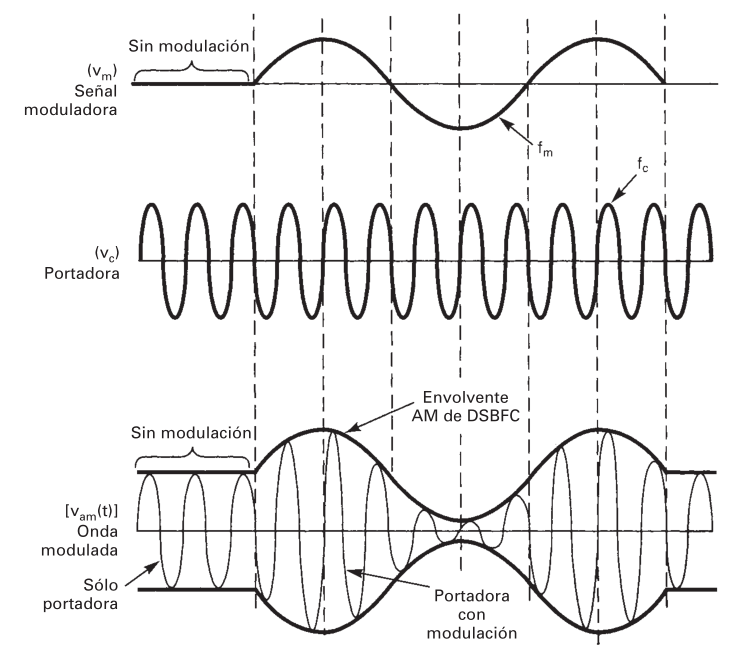
\includegraphics[scale=0.5]{screenshot001}
\end{center}
\subsection{Coeficiente de modulación}
Un termino que describe la cantidad de cambio de amplitud que hay en una forma de onda de AM es el coeficiente de modulación expresado como porcentaje. El porcentaje de modulación indica el cambio porcentual de amplitud de la onda de salida cuando sobre la portadora actúa una señal moduladora. Coeficiente de modulación es:
\begin{align}
	m=\frac{E_m}{E_c}
\end{align}
Donde m es el coeficiente de modulación, $E_m$ cambio máximo de amplitud de la forma de onda de voltaje de salida (volts), $E_c$ amplitud máxima del voltaje de la portadora no modulada (volts).
\subsection{Distribución de voltaje de AM}
Una portadora no modulada se puede describir matemáticamente con sigue:
\begin{align}
	v_c(t)=E_c \sin(2\pi f_c t)
\end{align}
La amplitud instantánea de la onda modulada se puede expresar como sigue:
\begin{align}
	v_am(t)=[E_c+E_m \sin (2\pi f_m t)][\sin(2\pi f_c t)]
\end{align}
sustituyendo $E_m$ por $mE_c$ y sacando factor común $E_c$:
\begin{align}
	v_{am}(t)=[1+m\sin(2\pi f_m t)][E_c\sin(2\pi f_c t)]
\end{align}
Desarrollando la ecuación anterior:
\begin{align}
	v_{am}(t)=E_c\sin(2\pi f_c t)-\frac{mE_c}{2}\cos[2\pi(f_c+f_m)t]+\frac{mE_c}{2}\cos[2\pi(f_c-f_m)t]
\end{align}
\begin{center}
	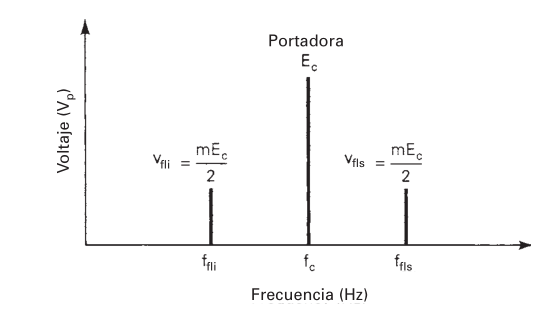
\includegraphics[scale=0.5]{screenshot002}
\end{center}
\subsection{Distribución de potencia en AM}
El promedio de la potencia disipada en una carga, por una portadora no modulada es igual al cuadrado del voltaje rms de la portadora, dividido entre la resistencia de carga. Esto se expresa:
\begin{align}
	P_c=\frac{(E_c)^2}{R(\sqrt{2})^2}=\frac{(E_c)^2}{2R}
\end{align}
Siendo $P_c$ potencia de la portadora (watts), $E_c$ voltaje máximo de la portadora (volts).
La potencia en las bandas laterales se determina por la siguiente ecuación:
\begin{align}
	P_{bls}=P_{bli}=\frac{(mE_c/2)^2}{2R}
\end{align}
La potencia total en una envolvente DSBFC de AM es:
\begin{align}
	P_t=P_c+P_{bls}+P_{bli}                   \\
	P_t=P_c+\frac{m^2P_c}{4}+\frac{m^2P_c}{4} \\
	P_t=P_c+\frac{m^2P_c}{2}                  \\
	P_t=P_c\left(1+\frac{m^2}{2}\right)
\end{align}
Se puede ver que la potencia de portadora en la onda modulada es igual que en la onda no modulada. Por tanto es evidente que la potencia de la portadora no se afecta en el proceso de modulación. La potencia total en la onda de AM es igual a la suma de las potencias de la portadora y de las bandas laterales, la potencia total en una envolvente de AM aumenta con la modulación.

\begin{center}
	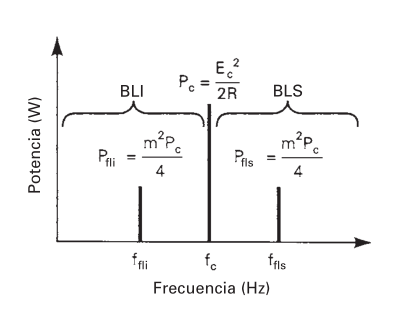
\includegraphics[scale=0.5]{screenshot003}
\end{center}
\subsection{Transmisor. Diagrama de bloques y espectro}
\begin{center}
	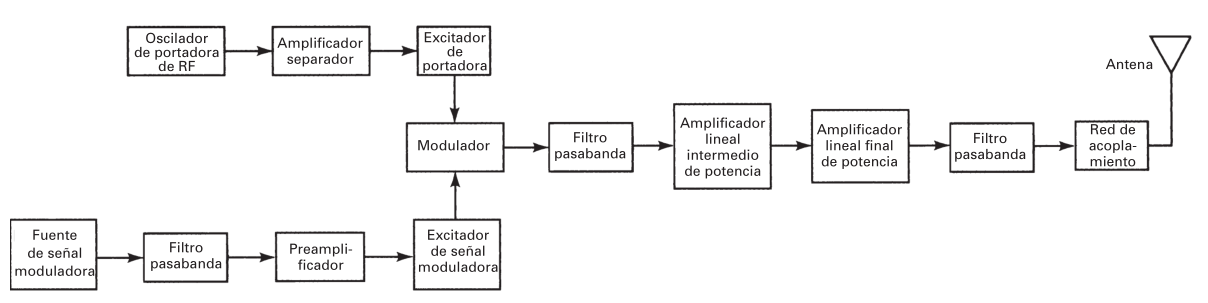
\includegraphics[scale=0.5]{screenshot004}
	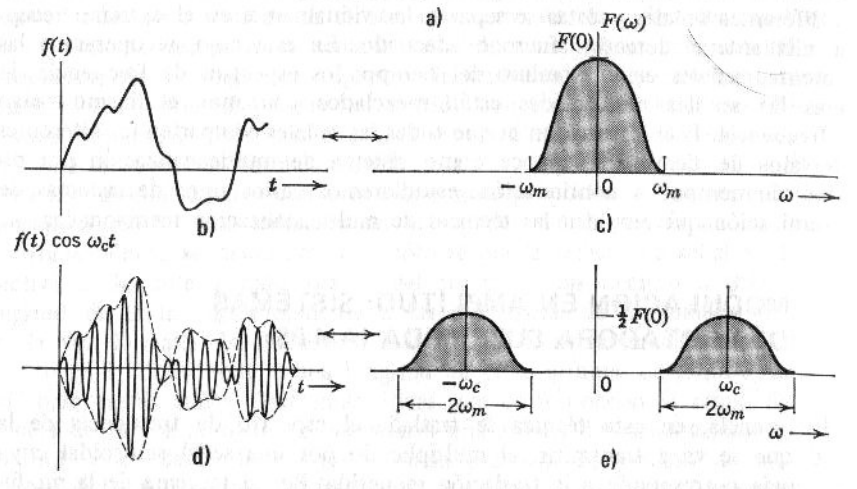
\includegraphics[scale=0.5]{screenshot005}
\end{center}

\section{Banda Lateral Única}
Los sistemas convencionales de AM usan el doble de ancho de banda que el necesario en los sistemas de banda lateral única. La información contenida en la banda superior es idéntica a la de la banda inferior, es una redundancia transmitir ambas bandas laterales.

\begin{center}
	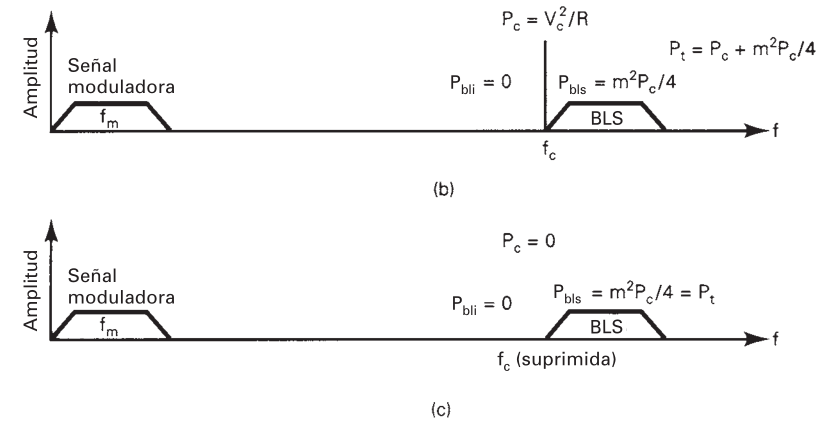
\includegraphics[scale=0.5]{screenshot006}
\end{center}

\subsection{AM de banda lateral única}
Es una forma de modulación de amplitud en la que la portadora se transmite con potencia máxima, pero solo se transmite una de las bandas laterales. Solo necesita la mitad del ancho de banda que la AM convencional. El cambio máximo en la envolvente es la mitad del que hay en la transmisión con doble banda lateral. Cuando baja el ancho de banda a la mitad, también se reduce a la mitad la potencia de ruido, y si se eliminar una banda lateral, la potencia en la parte de información de la onda también baja a la mitad, en consecuencia, las relaciones de señal a ruido con BLU y doble banda lateral son iguales.

\subsection{AM de banda lateral única y portadora suprimida}
Es una forma de modulación de amplitud en la que la portadora se suprime en su totalidad y se quita una de las bandas laterales. Por consiguiente, en SSBSC se requiere la mitad del ancho de banda que en la AM convencional de doble banda lateral, y bastante menos potencia de transmisión. Se puede apreciar que la potencia de la banda lateral es el 100\% de la potencia total transmitida.

\subsection{Banda lateral residual}
En este sistema las señales moduladoras de menor frecuencia se transmiten en doble banda lateral, y las de mayor frecuencia se transmiten en banda lateral única. La ventaja es que no se necesita un filtro tan abrupto.

\subsection{Ventajas de la transmisión con banda lateral única}
\textbf{Ahorro de energía} Se necesita mucho menor potencia transmitida para producir esencialmente la misma calidad de señal en el receptor que la que se alcanza con la transmisión con portadora de máxima potencia y doble banda lateral. En la portadora están al menos las dos terceras partes de la potencia de una señal normal de AM con doble banda lateral y portadora de máxima potencia, y la potencia máxima contenida en cualquiera de las bandas laterales solo es la sexta parte de la potencia.\\

\textbf{Ahorro de ancho de banda} En la transmisión de banda lateral única se requiere la mitad de ancho de banda que en la transmisión convencional de AM con doble banda lateral. Esto es una ventaja de bastante importancia en la actualidad, cuando el espectro de radiofrecuencias ya está sobresaturado.\\

\textbf{Reducción de ruido} En vista de que un sistema de banda lateral única usa la mitad del ancho de banda que la AM convencional, la potencia de ruido térmico se reduce a la mitad de la de un sistema con doble banda lateral. El sistema SSB tiene una ventaja en relación de señal a ruido de unos 12dB respecto a la AM convencional.\\

\subsection{Desventajas de la transmisión con banda lateral única}
\textbf{Receptores complicados} Los sistemas de banda lateral única requieren receptores mas complejos y costosos que los convencionales de AM, porque la mayoría de las transmisiones con banda lateral única tienen portadora reducida o suprimida. No se puede usar detección de envolvente a menos que se regenere la portadora a un nivel suficiente. Los receptores de banda lateral única requieren un circuito de recuperación y sincronizan de la portadora.\\

\textbf{Dificultades de sintonización} Los receptores de banda lateral única requieren una sintonización mas compleja y precisa que los receptores convencionales de AM. Esta desventaja se puede superar usando circuitos de sintonía más exactos, complejos y costosos.\\



\end{document}
